\documentclass[]{article}
\usepackage{lmodern}
\usepackage{amssymb,amsmath}
\usepackage{ifxetex,ifluatex}
\usepackage{fixltx2e} % provides \textsubscript
\ifnum 0\ifxetex 1\fi\ifluatex 1\fi=0 % if pdftex
  \usepackage[T1]{fontenc}
  \usepackage[utf8]{inputenc}
\else % if luatex or xelatex
  \ifxetex
    \usepackage{mathspec}
  \else
    \usepackage{fontspec}
  \fi
  \defaultfontfeatures{Ligatures=TeX,Scale=MatchLowercase}
\fi
% use upquote if available, for straight quotes in verbatim environments
\IfFileExists{upquote.sty}{\usepackage{upquote}}{}
% use microtype if available
\IfFileExists{microtype.sty}{%
\usepackage{microtype}
\UseMicrotypeSet[protrusion]{basicmath} % disable protrusion for tt fonts
}{}
\usepackage[margin=1in]{geometry}
\usepackage{hyperref}
\hypersetup{unicode=true,
            pdftitle={My Report},
            pdfauthor={Daniel Winkler},
            pdfborder={0 0 0},
            breaklinks=true}
\urlstyle{same}  % don't use monospace font for urls
\usepackage{longtable,booktabs}
\usepackage{graphicx,grffile}
\makeatletter
\def\maxwidth{\ifdim\Gin@nat@width>\linewidth\linewidth\else\Gin@nat@width\fi}
\def\maxheight{\ifdim\Gin@nat@height>\textheight\textheight\else\Gin@nat@height\fi}
\makeatother
% Scale images if necessary, so that they will not overflow the page
% margins by default, and it is still possible to overwrite the defaults
% using explicit options in \includegraphics[width, height, ...]{}
\setkeys{Gin}{width=\maxwidth,height=\maxheight,keepaspectratio}
\IfFileExists{parskip.sty}{%
\usepackage{parskip}
}{% else
\setlength{\parindent}{0pt}
\setlength{\parskip}{6pt plus 2pt minus 1pt}
}
\setlength{\emergencystretch}{3em}  % prevent overfull lines
\providecommand{\tightlist}{%
  \setlength{\itemsep}{0pt}\setlength{\parskip}{0pt}}
\setcounter{secnumdepth}{0}
% Redefines (sub)paragraphs to behave more like sections
\ifx\paragraph\undefined\else
\let\oldparagraph\paragraph
\renewcommand{\paragraph}[1]{\oldparagraph{#1}\mbox{}}
\fi
\ifx\subparagraph\undefined\else
\let\oldsubparagraph\subparagraph
\renewcommand{\subparagraph}[1]{\oldsubparagraph{#1}\mbox{}}
\fi

%%% Use protect on footnotes to avoid problems with footnotes in titles
\let\rmarkdownfootnote\footnote%
\def\footnote{\protect\rmarkdownfootnote}

%%% Change title format to be more compact
\usepackage{titling}

% Create subtitle command for use in maketitle
\newcommand{\subtitle}[1]{
  \posttitle{
    \begin{center}\large#1\end{center}
    }
}

\setlength{\droptitle}{-2em}
  \title{My Report}
  \pretitle{\vspace{\droptitle}\centering\huge}
  \posttitle{\par}
  \author{Daniel Winkler}
  \preauthor{\centering\large\emph}
  \postauthor{\par}
  \predate{\centering\large\emph}
  \postdate{\par}
  \date{May 14, 2018}


\begin{document}
\maketitle

\subsection{R Markdown}\label{r-markdown}

My text here\ldots{}. (see Gadea-Rivas, Gómez-Loscos, and Bandrés 2018,
18; Silverman 2018, 4)

Some more text, according to Gadea-Rivas, Gómez-Loscos, and Bandrés
(2018, 12). And another fact from a differnt page (2018, 25)

\begin{longtable}[]{@{}lrrr@{}}
\caption{Unemployment rate}\tabularnewline
\toprule
time & AT & DE & DK\tabularnewline
\midrule
\endfirsthead
\toprule
time & AT & DE & DK\tabularnewline
\midrule
\endhead
2006 & 5.3 & 10.1 & 3.9\tabularnewline
2007 & 4.9 & 8.5 & 3.8\tabularnewline
2008 & 4.1 & 7.4 & 3.4\tabularnewline
2009 & 5.3 & 7.6 & 6.0\tabularnewline
2010 & 4.8 & 7.0 & 7.5\tabularnewline
2011 & 4.6 & 5.8 & 7.6\tabularnewline
2012 & 4.9 & 5.4 & 7.5\tabularnewline
2013 & 5.4 & 5.2 & 7.0\tabularnewline
2014 & 5.6 & 5.0 & 6.6\tabularnewline
2015 & 5.7 & 4.6 & 6.2\tabularnewline
2016 & 6.0 & 4.1 & 6.2\tabularnewline
2017 & 5.5 & 3.8 & 5.7\tabularnewline
\bottomrule
\end{longtable}

\subsection{Including Plots}\label{including-plots}

You can also embed plots, for example:

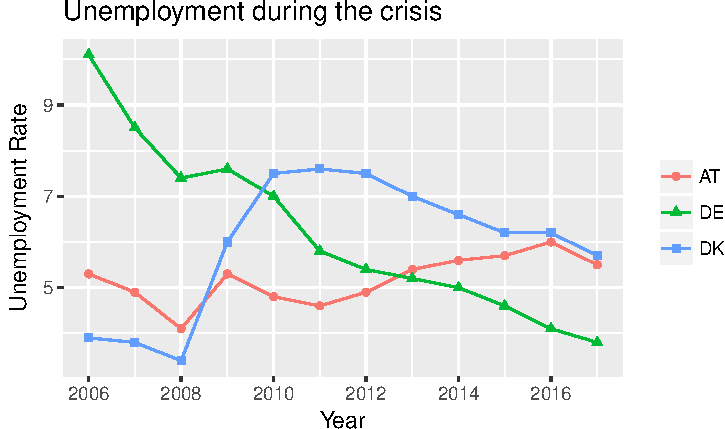
\includegraphics{markdownIntro_files/figure-latex/pressure-1.pdf}

\subsection{Some Math}\label{some-math}

\[
u = \alpha + \beta_1 i + \beta_2 \pi + \beta_3 y + \varepsilon
\]

\(\beta\) is great!

\subsection*{References}\label{references}
\addcontentsline{toc}{subsection}{References}

\hypertarget{refs}{}
\hypertarget{ref-gadea18}{}
Gadea-Rivas, M Dolores, Ana Gómez-Loscos, and Eduardo Bandrés. 2018.
``Clustering Regional Business Cycles.'' \emph{Economics Letters} 162.
Elsevier: 171--76.

\hypertarget{ref-silverman18}{}
Silverman, Bernard W. 2018. \emph{Density Estimation for Statistics and
Data Analysis}. Routledge.


\end{document}
